
\subsection{Analytical solution}

As we have previously seen, Péclet's number is defined as
\begin{equation}
	\mathrm{Pe} = 
	\frac{\text{convection transport rate}}{\text{diffusion transport rate}} = 
	\frac{\rho u L}{\Gamma}
\end{equation}
Note that the factor $\beta$ in the PDE from problem \eqref{eq:diagonal_case_cauchy_problem} is a constant determined by the geometry, whereas Peclet's number depends on the fluid and on the velocity field. Since no more factors intervene on the PDE, this tells us that the behaviour of the solution will depend greatly on Peclet's number. 

\subsubsection{Analytical solution for \texorpdfstring{$\mathrm{Pe} = \infty$}{infinite Péclet's number}}

Whenever $\mathrm{Pe} \to +\infty$, it implies $\Gamma \to 0^+$ since infinite values for the density, velocity or characteristic length make no physical sense. Therefore the difussion coefficient tends to $0$, which means the Laplacian term, linked to the diffusion process, is negligible. Dividing the PDE from \eqref{eq:diagonal_case_cauchy_problem} by Péclet's number results in the following Cauchy problem:
\begin{equation} \label{eq:diagonal_case_cauchy_problem_infinite_peclet}
	\left\{
	\begin{aligned}
		&\pdv{\phi}{x} + \pdv{\phi}{y} = 0 &
		&\text{in } \Omega \\
		&\phi = g &
		&\text{on } \partial \Omega
	\end{aligned}
	\right.
\end{equation}
The PDE \eqref{eq:diagonal_case_cauchy_problem_infinite_peclet} is known as the transport equation, which is a first order linear PDE. In our case it has constant coefficients, making it easier to solve analitically.

\begin{definition}
	A classical solution to \eqref{eq:diagonal_case_cauchy_problem_infinite_peclet} is a function $\phi \colon \overline{\Omega} \rightarrow \real$ that satisfies:
	\begin{enumerate}[label={(\roman*)}, topsep=0pt]
		\item $\phi \in \mathcal{C}^1(\Omega) \cap \mathcal{C}(\overline{\Omega})$, \ie $\phi$ is differentiable with continuity in $\Omega$ and continuous up to the boundary,
		\item $\phi$ satisfies the PDE, and
		\item $\phi$ satisfies the boundary conditions.
	\end{enumerate}
\end{definition}
In order to find the solution to \eqref{eq:diagonal_case_cauchy_problem_infinite_peclet}, we will assume $\phi$ is a $\mathcal{C}^1(\Omega) \cap \mathcal{C}(\overline{\Omega})$ function. Once we find the solution, we will be able to tell whether $\phi$ is a classical solution, or otherwise give a meaning to $\phi$.

We introduce some notation that will be useful. Given $m$ vectors $\vb{w}_1, \ldots, \vb{w}_m \in \real^n$, the set $[\vb{w}_1, \ldots, \vb{w}_m] = \{ \sum_{i=1}^m \lambda_i \vb{w}_i \mid \lambda_1, \ldots, \lambda_m \in \real \}$ is the vector subspace of $\real^n$ spanned by $\vb{w}_1, \ldots, \vb{w}_m$. If $W \subset \real^m$ is a vector subspace, $W^\perp = \{ v \in \real^n \mid v \vdot w = 0 \ \forall w \in W \}$ is the vector subspace orthogonal to $W$.

To deduce the solution to \eqref{eq:diagonal_case_cauchy_problem_infinite_peclet} we shall follow the method of characteristics. Using the gradient of $\phi$ we can write the PDE as
\begin{equation} \label{eq:diagonal_case_cauchy_problem_infinite_peclet_orthogonal_vectors}
	\left( 1, 1 \right)
	\vdot
	\grad{\phi} = 
	\left( 1, 1 \right)
	\vdot
	\begin{pmatrix}
	\displaystyle\pdv{\phi}{x} \\[10pt] \displaystyle\pdv{\phi}{y}
	\end{pmatrix} = 
	\pdv{\phi}{x} + \pdv{\phi}{y} = 0
\end{equation}
Recall from vector calculus that the gradient vector of $\phi$ gives the direction of maximum growth of $\phi$ at each point, whilst a non--zero vector $\vb{w} \in [\grad{\phi}(x,y)]^\perp$ provides the direction at $(x,y)$ along which $\phi$ remains constant. Equation \eqref{eq:diagonal_case_cauchy_problem_infinite_peclet_orthogonal_vectors} tells us than $\phi$ is constant along the direction given by $(1, 1)$. To check this, we may exploit the fact that the PDE is first--order linear and use the chain rule to rewrite \eqref{eq:diagonal_case_cauchy_problem_infinite_peclet_orthogonal_vectors}. Let $I \subset \real$ be an open interval and let $h \equiv (h_1, h_2) \colon I \subset \real \rightarrow \Omega \subset \real^2$, $s \mapsto h(s) = (h_1(s), h_2(s))$ be a $\mathcal{C}^1$ mapping such that $h_1' = h_2' = 1$. The image of $h$, $C = \image{h} = \{ (x, y) \in \real^2 \mid x = h_1(s), \, y = h_2(s), \, s \in I \} \subset \Omega$ is a $\mathcal{C}^1$ curve in $\real^2$. The restriction of $\phi$ to  $C$, given by $\varphi = \phi \circ h \colon \real \rightarrow \real$, is also a $\mathcal{C}^1$ function. By the chain rule,
\begin{equation} \label{eq:diagonal_case_cauchy_problem_infinite_peclet_chain_rule}
	\frac{\dd}{\dd{s}} \varphi(s) = 
	\frac{\dd}{\dd{s}} \phi(h_1(s), h_2(s)) = 
	\frac{\partial \phi}{\partial x} (h_1(s), h_2(s)) \, h_1'(s) + 
	\frac{\partial \phi}{\partial y} (h_1(s), h_2(s)) \, h_2'(s) =
	\frac{\partial \phi}{\partial x} + \frac{\partial \phi}{\partial y} = 0
\end{equation}
which implies that $\phi$ is constant on $C \subset \Omega$. Now we would like to find $C$. By hypothesis, we have $h_1' = h_2' = 1$. Moreover, the component functions of $h$ can be interpreted as the coordinates of a point in $\real^2$, that is $(h_1(s), h_2(s)) = (x, y)$. Given this information, we can pose the following Cauchy problem:
\begin{equation} \label{eq:diagonal_case_cauchy_problem_infinite_peclet_characteristics_problem}
	\left\{
	\begin{aligned}
		&h'(s) = (h_1'(s), h_2'(s)) = (1, 1) & &\text{in } I \subset \real \\
		&h(0) = (h_1(0), h_2(0)) = (x_0, y_0)
	\end{aligned}
	\right.
\end{equation}
The solution to \eqref{eq:diagonal_case_cauchy_problem_infinite_peclet_characteristics_problem} exists and is unique due to theorem \ref{teo:picard_lindelof}, and is given by
\begin{equation}
	h(s) = (x_0 + s, y_0 + s) = (x_0, y_0) + s(1, 1)
\end{equation}
The point $(x_0, y_0) \in \real^2$ is arbitrary, but it should be chosen so that it eases finding the solution to \eqref{eq:diagonal_case_cauchy_problem_infinite_peclet}. Since part of the information of the solution is given by the boundary conditions, we may choose the point to be on the boundary. Therefore the curve along which $\phi$ is constant is not a single curve, but rather a family of curves given by
\begin{equation}
	h(s; x_0, y_0) = (x_0, y_0) + s(1, 1), \quad (x_0, y_0) \in \partial \Omega
\end{equation}
or in implicit form by the equation
\begin{equation} \label{eq:diagonal_case_cauchy_problem_infinite_peclet_characteristics_implicit_form}
	x - y = x_0 - y_0, \quad (x_0, y_0) \in \partial \Omega
\end{equation}
These curves are named characteristic curves or simply characteristics. Some of them are represented in figure \ref{fig:diagonal_case_cauchy_problem_infinite_peclet_characteristics_problem}. As it can be seen, the characteristics have implicit equation $x - y = c$ with $c \in [-L, L]$.

\begin{figure}[h]
	\centering
	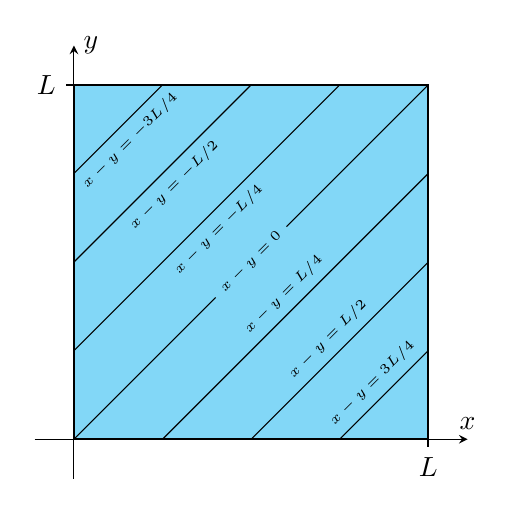
\begin{tikzpicture}
		% Lenghts
		\def\alength{5}
		\def\L{4.5}
		\def\mlength{0.1}
		% Axis
		\draw[-stealth] (0,-0.5) -- (0,\alength) node[right]{$y$};
		\draw[-stealth] (-0.5,0) -- (\alength,0) node[above]{$x$};
		\draw[black, thick] (\L,0) -- ++(0,-\mlength) node[below]{$L$};
		\draw[black, thick] (0,\L) -- ++(-\mlength,0) node[left]{$L$};
		% Domain
		\fill[cyan!70!white,opacity=0.7] (0,0) rectangle (\L, \L);
		\draw[thick, thick] (0,0) rectangle (\L, \L);
		% Characteristics
%		\draw[black] (0,0) -- node[midway, above, rotate=45]{\tiny{$x - y = 0$}} (\L, \L);
		\node[rotate=45] at ({0.5*\L}, {0.5*\L}) {\tiny{$x - y = 0$}};
		\draw[black] (0,0) -- ({0.4*\L}, {0.4*\L});
		\draw[black] ({0.6*\L}, {0.6*\L}) -- (\L, \L);
		
		\draw[black] ({0.25*\L}, 0) -- node[midway, above, rotate=45]{\tiny{$x - y = L/4$}} 
		(\L, {0.75*\L});
		\draw[black] ({0.50*\L}, 0) -- node[midway, above, rotate=45]{\tiny{$x - y = L/2$}} 
		(\L, {0.50*\L});
		\draw[black] ({0.75*\L}, 0) -- node[midway, above, rotate=45]{\tiny{$x - y = 3L/4$}} 
		(\L, {0.25*\L});
		
		
		
		\draw[black] (0, {0.25*\L}) -- node[midway, below, rotate=45]{\tiny{$x - y = -L/4$}} 
		({0.75*\L}, \L);
		\draw[black] (0, {0.50*\L}) -- node[midway, below, rotate=45]{\tiny{$x - y = -L/2$}} 
		({0.50*\L}, \L);
		\draw[black] (0, {0.75*\L}) -- node[midway, below, rotate=45]{\tiny{$x - y = -3L/4$}} 
		({0.25*\L}, \L);
	\end{tikzpicture}
	\caption{Some characteristics of problem \eqref{eq:diagonal_case_cauchy_problem_infinite_peclet}.}
	\label{fig:diagonal_case_cauchy_problem_infinite_peclet_characteristics_problem}
\end{figure}

\noindent
Intuitively, the characteristics give the paths in $\real^2$ through which the information of the boundary conditions is transported. Notice that each characteristic starting on $C_1$ ends on $C_1$, and the same holds for $C_2$. Moreover, by definition of the Cauchy problem, $\phi$ is constant on $C_1$ and on $C_2$. Therefore the value of $\phi$ on the characteristic $x - y = c$ is the value that $g$ takes on the part of the boundary the characteristic intersects:
\begin{equation} \label{eq:diagonal_case_cauchy_problem_infinite_peclet_solution}
	\phi(x,y) = 
	\left\{
	\begin{aligned}
		&g(x-y) = \phi_\text{low} 	& &\text{if } x - y \geq 0 \\
		&g(y-x) = \phi_\text{high} 	& &\text{if } x - y < 0
	\end{aligned}
	\right.
	\quad
	(x, y) \in \overline{\Omega}
\end{equation}
Notice that it is not necessary to prescribe boundary conditions on $(0, L] \times \{ L \}$ nor on $\{ L \} \times (0, L)$, since the value of the solution on those parts of the boundary is already given by the value $\phi$ takes on $[0, L] \times \{ 0 \} \cup \{ 0 \} \times (0, L]$.


Now we check our initial assumption that $\phi \in \mathcal{C}^1(\Omega) \cap \mathcal{C}(\overline{\Omega})$. If $\phi_\text{low} = \phi_\text{high}$ the solution \eqref{eq:diagonal_case_cauchy_problem_infinite_peclet_solution} is constant and therefore is a solution in the classical sense.

\begin{theorem}
	Assume $\phi_\text{low} = \phi_\text{high}$. Then the solution to problem \eqref{eq:diagonal_case_cauchy_problem_infinite_peclet} exists, is unique and is a solution in the classical sense.
\end{theorem}
\begin{proof}
	We have proved the existence of a solution by giving formula \eqref{eq:diagonal_case_cauchy_problem_infinite_peclet_solution}. The uniqueness comes from the method of characteristics we have followed. In it we have seen that $\phi$ is constant on the characteristic curves and then we have found the equation of characteristics. These curves are unique due to the Theorem of Existence and Uniqueness of solutions to ODEs. Finally $\phi$ is a $\mathcal{C}^1(\Omega) \cap \mathcal{C}(\overline{\Omega})$ function because it is constant on $\overline{\Omega}$.
\end{proof}

Assume that $\phi_\text{low} < \phi_\text{high}$. Then $\phi$ is not continuous on the segment $\{ x - y = 0 \} \cap \overline{\Omega}$ whence it cannot be a differentiable function. Notice that to find the function \eqref{eq:diagonal_case_cauchy_problem_infinite_peclet_solution} it was not necessary to prescribe boundary conditions on $(0, L] \times \{ L \}$ nor on $\{ L \} \times (0, L)$, since the value of the solution on those parts of the boundary is already given by the value $\phi$ takes on $[0, L] \times \{ 0 \} \cup \{ 0 \} \times (0, L]$. In order to give a meaning to function \eqref{eq:diagonal_case_cauchy_problem_infinite_peclet_solution} we will formulate a similar problem to \eqref{eq:diagonal_case_cauchy_problem_infinite_peclet}. Let $D_1 = [0, L] \times \{ 0 \}$, $D_2 = \{ 0 \} \times (0, L]$, and let $\tilde{g} \colon D_1 \cup D_2 \rightarrow \real$ be defined by
\begin{equation}
	\tilde{g}(x,y) = 
	\left\{
	\begin{aligned}
		&\phi_\text{low}	& &\text{if } (x,y) \in D_1 \\
		&\phi_\text{high} 	& &\text{if } (x,y) \in D_2
	\end{aligned}
	\right.
\end{equation}
Consider the following Cauchy problem:
\begin{equation} \label{eq:diagonal_case_cauchy_problem_infinite_peclet_weak}
	\left\{
	\begin{aligned}
		&\pdv{\phi}{x} + \pdv{\phi}{y} = 0 &
		&\text{in } \Omega \\
		&\phi = \tilde{g} &
		&\text{on } D_1 \cup D_2
	\end{aligned}
	\right.
\end{equation}
It is essentially the same problem as \eqref{eq:diagonal_case_cauchy_problem_infinite_peclet} but without prescribing boundary conditions on the right and top boundaries. It can be checked that the solution to \eqref{eq:diagonal_case_cauchy_problem_infinite_peclet_weak} found by following the method of characteristics is also given by \eqref{eq:diagonal_case_cauchy_problem_infinite_peclet_solution}. But we again encounter the problem to give a meaning to the derivatives, since \eqref{eq:diagonal_case_cauchy_problem_infinite_peclet_solution} is not continuous on $\overline{\Omega}$. 

\begin{definition}
	A function $\psi \colon \overline{\Omega} \rightarrow \real$ is said a weak solution of \eqref{eq:diagonal_case_cauchy_problem_infinite_peclet} if 
	\[
		\int_\Omega 
	\]
\end{definition}

\subsubsection{Analytical solution for \texorpdfstring{$\mathrm{Pe} = 0$}{zero Péclet's number}}

Now we consider the problem \eqref{eq:diagonal_case_cauchy_problem} when $\mathrm{Pe} \to 0$. Since $\rho > 0$ and $L > 0$, the fact that Péclet's number is close to zero implies that velocity $u$ is close to zero. In the extreme case when $u = 0$, there is no transport, therefore $\mathrm{Pe} = 0$ and problem \eqref{eq:diagonal_case_cauchy_problem} becomes
\begin{equation} \label{eq:diagonal_case_cauchy_problem_zero_peclet}
	\left\{
	\begin{aligned}
		&\Delta \phi = 0 &
		&\text{in } \Omega \\
		&\phi = g &
		&\text{on } \partial \Omega
	\end{aligned}
	\right.
\end{equation}
which is Laplace's problem in the square $\Omega$. 

\subsubsection{General problem}

Hereafter we consider problem \eqref{eq:diagonal_case_cauchy_problem} with $0 < \mathrm{Pe} < +\infty$ with $\phi_\text{low} < \phi_\text{high}$. A classical solution to \eqref{eq:diagonal_case_cauchy_problem} is a function $\phi \in \mathcal{C}^2(\Omega) \cap \mathcal{C}(\overline{\Omega})$, \ie a twice differentiable function with continuity which is continuous up to the boundary as well, that satisfies the PDE and the boundary conditions. The function $g$ giving the boundary conditions is not continuous at $(0,0)$ nor at $(L, L)$ unless $\phi_\text{low} = \phi_\text{high}$. Therefore problem \eqref{eq:diagonal_case_cauchy_problem} cannot have a classical solution. Nonetheless it might have a solution in the weak sense.

Before studying the theorem that deals with the existence of a weak 

\begin{definition}
	contenidos...
\end{definition}

\subsubsection{Expected nature of the solution}